\documentclass[twoside]{article}
\usepackage{ecj,palatino,epsfig,latexsym,natbib}
\usepackage{float} % lets you have non-floating floats
\usepackage{url} % for typesetting urls
\usepackage{graphicx} % for including images
\usepackage{caption}
\usepackage{program}
\usepackage{tabularx}
\usepackage{colortbl}

\usepackage{amsmath,amssymb}
%\usepackage{mathtools}
\usepackage{etoolbox}
\usepackage{hhline}
\usepackage{subcaption}
\newfloat{fig}{thp}{lof}[section]
\floatname{fig}{Figure}
\let\bbordermatrix\bordermatrix
\patchcmd{\bbordermatrix}{8.75}{4.75}{}{}
\patchcmd{\bbordermatrix}{\left(}{\left[}{}{}
\patchcmd{\bbordermatrix}{\right)}{\right]}{}{}


%% do not add any other page- or text-size instruction here

\parskip=0.00in

\begin{document}

\ecjHeader{x}{x}{xxx-xxx}{201X}{45-character paper description goes here}{Tan, Ma, Zhang}
\title{\bf Optimization of Location Allocation of Web Service using non-dominated sorting algorithm(NSGA-II)
}  

\author{\name{\bf Boxiong Tan} \hfill \addr{tanboxi@ecs.vuw.ac.nz}\\ 
        \addr{Department of Science and Engineering, Victoria of Wellington, 
        Wellington, Zip, New Zealand}
\AND
       \name{\bf Hui Ma} \hfill \addr{hui.ma@ecs.vuw.ac.nz}\\
        \addr{Department of Science and Engineering, Victoria of Wellington, 
		Wellington, Zip, New Zealand}
}

\maketitle

\begin{abstract}

The abstract goes here.  It should be about 200 words and give the
reader a summary of the main contributions of the paper.   
Remember that readers may decide to read or not to read your
paper based on what is in the abstract.  The abstract never
contains references.  

\end{abstract}

\begin{keywords}

Genetic algorithms, 
evolutionary programming,
NSGA-II,
multiobjective.

\end{keywords}
\section{Introduction}
Web Services are considered as self-contained, self-describing, modular applications that can be published, located, and invoked across the Web \cite{Ran:2003:MWS:844357.844360}. 
In recent years, web services technology is becoming increasingly popular because the convenience, low cost and capacity to be composed into high-level business processes \cite{Aboolian200964}.


With the ever increasing number of functional similar web services being available on the Internet, the web service providers (WSPs) are trying to improve the quality of service (QoS) to become competitive in the market.  
QoS also known as non-functional requirements to  web services, is the degree to which a service meets specified requirements or user needs \cite{4061431}, such as response time, security and availability. 
Among numerous QoS measurements, service response time is a critical factor for many real-time services, e.g. traffic service or finance service. 
Service response time has two components: transmission time (variable with message size) and network latency \cite{Johansson:2000:INL:595252.595281}. 
Study \cite{Johansson:2000:INL:595252.595281, 916684} has shown that network latency is a significant component of service response delay.
Ignoring network latency will underestimate response time by more than 80 percent. Since network latency is related to network topology as well as physical distance \cite{distanceMetrics}. 
The network latency could also vary with the network topology changes.
The only way to reduce the network latency is move the service to a location where has smaller network latency to the user center. 
Hence, the WSPs need to consider which physical location to deploy their services so that it could minimize the cost as well as ensure the QoS.

The Web service location-allocation problem is essentially a multi-objective optimization problem \cite{Multiobjective}.
Because of the confliction between service quality and deployment cost. 
Ideally, WSP could deploy their services to each user center in order to provide the best quality.
That is, the more services deployed, the better the quality and the higher cost. 
This problem is considered as an NP-hard due to the fact that the combinatorial explosion of the search space \cite{Vanrompay:2008:GAO:1387309.1387313}. 


Very few researches \cite{Aboolian200964, Sun:2006:LMW:1217741.1217754} study this problem.
Both studies try to solve the problem by integer linear programming techniques.
However, integer programming techniques do not scale well, so that no satisfactory results can be obtained for large-scale datasets. 

Evolutionary algorithms (EAs) have been used in solving multi objective optimization problems in recent years. 
EAs are ideal for solving multi objective optimization problems \cite{key:article}, since EA works with a population of solutions, a simple EA can be extended to maintain a diverse set of solutions.
With an emphasis for moving toward the true Pareto-optimal region, an EA can be used to find multiple Pareto-optimal solutions in one single simulation run \cite{OptimizationElectrical}.

Hai \cite{EnhancedGenetic} proposed an enhanced genetic algorithm-based approach which make use of the integer scalarization technique to solve the multi-objective problem.
The genetic algorithm (GA) is an EA that uses genetic operators to obtain optimal solutions without any assumptions about the search space.
This algorithm solve the scalability problem in the dataset, however the integer scalarization technique \cite{Multiobjective} has some disadvantages: 

\begin{enumerate}
	\item The decision maker needs to choose an appropriate weights for the objectives to retrieve a satisfactorily solution.
	\item The algorithm does not produce an uniform spread of points on the Pareto curve. That is, all points are grouped in certain parts of the Pareto front.
	\item Non-convex parts of the Pareto set cannot be reached by minimizing convex combinations of the object functions.
\end{enumerate}

Evolutionary multi objective optimization (EMO) methodologies on the other hand, successfully avoid the above mentioned problems and demonstrated their usefulness in find a well-distributed set of near Pareto optimal solutions \cite{Aboolian200964}. Non-dominated sorting GA (NSGA-II) \cite{996017}, Strength Pareto Evolutionary Algorithm 2 (SPEA-2) \cite{Deb:2005:EED:1109044.1109049} have become standard approaches. 
Some schemes based on particle swarm optimization approaches \cite{Elhossini:2010:SPP:1739146.1739151, Huang:2006:CLP:1108677.1108683} are also important. 
Among numerous EA approaches, NSGA-II is one of the most widely used methods for generating the Pareto frontier. 
NSGA-II implements elitism and uses a phenotype crowd comparison operator that keeps diversity without specifying any additional parameters \cite{Deb06referencepoint}.
In our approach, we apply a modified version of NSGA-II since the web service location-allocation is a discrete problem. 

In this paper we consider the problem faced by a WSP who has existing facilities but wishes to use the collected data to re-allocate their services in order to maximum their profit.
The WSP must decide on facility locations from a finite set of possible locations. 
In order to make the decision, the WSP must first analyze the data which were collected from current services. 
The collected data should includes the records of invocation from each unique IP address.
Therefore, based on these data, the WSP could summarize several customer demand concentrated at \textit{n} discrete nodes \cite{Aboolian200964}, namely user centers. 
We assume the WSP has already done this step and list of user centers and candidate service deployment locations are given.
In addition to decide which location to re-allocate the services, a dataset which contains the network latency between demand user center and candidate location are critical. 
The WSP could collect the data or use existed dataset \cite{5552800, 6076756}. 
Then, the service provider could use the algorithm which proposed by this paper, to select an optimal plan based on their funds. 
The algorithm will produce a near optimal solution which indicate the services deployment locations with a minimum cost and best service quality.
The main objectives are:
\begin{itemize}
	\item To model the web service location-allocation problem so that it can be tackled with NSGA-II
	\item To develop a modified NSGA-II approach for the web service location-allocation problem
	\item To evaluate our approach by comparing it to a GA approach which use integer scalarization technique.
\end{itemize}











\section{Problem Description}
\subsection{Model formulation}
The problem is to determine which facility locations that could maximus WSPs’ profit 
as well as ensure low network latency. 
Let $S = \{ 1, 2, ..., s\}$ be the set of services. We assume that the demand for service is concentrated at $i$ 
demand nodes $I = \{ 1, 2, ..., i \}$. Let $J = \{ 1, 2, ..., j \}$ be the set of $j$ candidate facility locations.
To model the service location-allocation problem we use four matrices: service network latency matrix $L$, service location
matrix $A$, service invocation frequency matrix $F$ and cost matrix $C$.

The server network latency matrix $L = [l_{ij}]$, is used to record network latency from user centers to 
candidate locations, where $l_{ij}$ is a real number denotes the network latency from user center $i$ to candidate 
location $j$. 
These data could be retrieved from implementing a network latency experiment or using existed datasets \cite{5552800, 6076756}.
\begin{center}
$
L = \bbordermatrix{~ & j_{1} & j_{2} & j_{3} & j_{4} \cr
					i_{1}	&5.09 &2.37 &4.01	&3.9	\cr
					i_{2}	&0.8  &2.9 &3.2	&1.2 \cr
					i_{3}	&2.74 &1.2 &5.3	&0.95 \cr} 
$
\end{center}
The service location matrix $A = [y_{sj}]$ represents the actual service location-allocation, where $y_{sj}$  is a binary value ( i.e., 1 or 0) shows whether a service $s$ is deployed in candidate location $j$ or not.
We use the service location matrix A as the representation of chromosome that evolve itself during the progress.
\begin{center}
$
A = \bbordermatrix{~ & j_{1} & j_{2} & j_{3} & j_{4} \cr
					s_{1}	&0 &1 &0	&0	\cr
					s_{2}	&0  &0 &1	&1 \cr
					s_{3}	&1 &1 &0	&0 \cr} 
$
\end{center}

The service invocation frequency matrix $F= [f_{is}]$, is used to record services invocation frequency from user centers, which $f_{is}$ is an integer that indicate the number of invocation in a period of time from user center $i$ to service s. e.g. 120 invocations per day from user center $i_{1}$ to $s_{1}$.
\begin{center}
$
F = \bbordermatrix{~ & s_{1} & s_{2} & s_{3}  \cr
					i_{1}	&120 &35 &56	\cr
					i_{2}	&14  &67 &24 \cr
					i_{3}	&85 &25 &74 \cr} 
$
\end{center}

The cost matrix $C = [c_{sj}]$, is used to record the cost of deployment of services from candidate locations, 
which $c_{sj}$ is an integer that indicate the cost of the deployment fee from a candidate location. 
e.g 130 \$ to deploy $s_{1}$ from $j_{1}$.
\begin{center}
$
C = \bbordermatrix{~ & j_{1} & j_{2} & j_{3} & j_{4} \cr
					s_{1}	&130 &80 &60	&68	\cr
					s_{2}	&96  &52 &86	&78 \cr
					s_{3}	&37 &25 &54	&46 \cr} 
$
\end{center}

Consider the following key modeling assumptions:
\begin{enumerate}
	\item The new WSP decides where to locate his facilities regardless if there is existed functional similar services from other WSPs.
	\item This choice is made only consider two factors: total network latency and total cost.
	\item We assume a fixed customer allocation policy for WSPs. In practice, Web Services typically offer clients persistent and interactive services, which often span over multiple sessions. Therefore, a dynamic reallocation scheme is not practical as it may disrupt the continuity of the services.
\end{enumerate}

\subsection{Discreted NSGA-2 algorithm}
NSGA-2 belong to the larger class of evolutionary algorithms (EAs), which generate approximate solutions to 
optimization and search problems by using techniques inspired by the principles of natural 
evolution: selection, crossover and mutation.

The steps involved in the solution of optimization problem using NSGA-II are summarized as follows.
\begin{itemize}
	\item Population initialization
	\item Non-dominated sort
	\item Crowding distance
	\item Selection
	\item Genetic operators
		\begin{enumerate}
			\item crossover
			\item mutation
			\item repair operators
		\end{enumerate}
	\item Recombination and selection
\end{itemize}

\subsection{Chromosome Representation}
In our problem, the chromosome is the service location matrix A that we mentioned in the previous section. 
\subsection{Objectives and Fitness Function}
The objective functions of this entire problem are following:
\begin{itemize}
	\item Minimize the total cost of services. n is the number of service, m is the number of candidate location.
		\begin{center}
			\begin{equation}
				CostFitness = \sum\limits_{s \in S} \sum\limits_{j \in J} C_{sj} \times A_{sj}
			\end{equation}
		\end{center}
	\item Minimize the network total latency of the services.
		\begin{itemize}
			\item For each chromosome, firstly, calculate the number of invocation for each service.
				\begin{center}
					$Invocation_{s} = \sum\limits_{i \in I} F_{is}$
				\end{center}
			\item Calculate the total number of each services.
				\begin{center}
					$ServiceNo_{s} = \sum\limits_{j \in J} A_{sj}$
				\end{center}
			\item Divide Invocations by Service in order to calculate the average invocation for each location.
				\begin{center}
					$AverageInvocation_{i} = Invocation_{s} \div ServiceNo_{s}$
				\end{center}

			\item Calculate the latency of each service by multiply latency matrix $L$ by service allocation matrix $A$(chromosome).
				\begin{center}
					$LocationLatency_{i} = \sum\limits_{i \in I} L_{ij} \times A_{sj}$
				\end{center}

			\item Calculate the total latency of the multiplication of AverageInvocationi and $LocationLatency_{i}$.
				\begin{center}
					\begin{equation}
						LatencyFitness = \sum\limits_{i \in I} AverageInvocation_{i} \times LocationLatency_{i}
					\end{equation}
				\end{center}
		\end{itemize}
\end{itemize}
The population is initialized based on the problem range and constraints. 
In our problem, we have two constraints, the cost constraint and latency constraint. 
If the initialized chromosome does not satisfy the constraints, then repair operators will attempt to 
recover from possible constraint violations. The detail of repair operators will be discuss in section 2.5.2.
\subsection{Constraints}
The our approach, each chromosome have to satisfy two constraints to be a feasible solution.
The first constraint controls the service number which is make sure that each service is deployed in at 
least one location.
\begin{center}
	\begin{equation}
		\sum\limits_{s \in S} A_{sj} \geq 1
	\end{equation}
\end{center}

The second constraint is cost constraint which predefined the upper boundary of the total cost.
An integer number CostLimitation is defined. This constraint will try to constraints
\begin{center}
	\begin{equation}
		\sum\limits_{s \in S} \sum\limits_{j \in J} C_{sj} \times A_{sj} \leq CostLimitation
	\end{equation}
\end{center}
The constraint is implemented by repair operators which is introduced in the next section.

\subsection{Genetic operators}
Specific selection, mutation and crossover operators were implemented. It is important to note that mutation and 
crossover operators can produce solutions that might violate the constraints. Therefore, repair 
operators are needed to try to maintain feasible solutions. The original NSGA-II use a simulated 
binary crossover (SBX) \cite{930314} and polynomial mutation \cite{Raghuwanshi04} to cope with continuous problem. 
However, our problem is discretized, therefore we use the regular GA mutation and crossover.


\subsubsection{Mutation}
The mutation operator works as follows: Initially choose one random location from the chromosome. 
Then, reverse the bit, e.g. 0 to 1 or 1 to 0. 

In this study, a chromosome in a population will be selected based on mutation possibility $P_{m}$. 
As shown in below, a random position will be selected and replaced by a reversed number.
\begin{figure}[ht]
\centering
	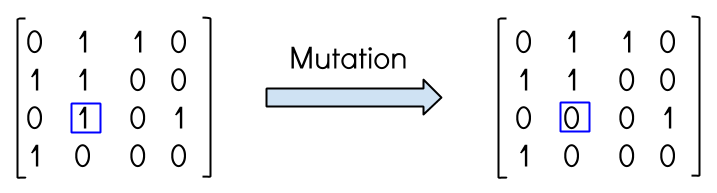
\includegraphics[width=0.5\textwidth]{pics/mutation.png}
\caption{}
\label{graph1}
\end{figure}
\subsubsection{Crossover}
The crossover operator in this paper is the single point crossover. 
The crossover is controlled by crossover probability $P_{c}$. 
The crossover point is created randomly within the length of the chromosome. 
As in the example below, two parents crossover at point X, then two offspring were generated.
\begin{figure}[ht]
\centering
	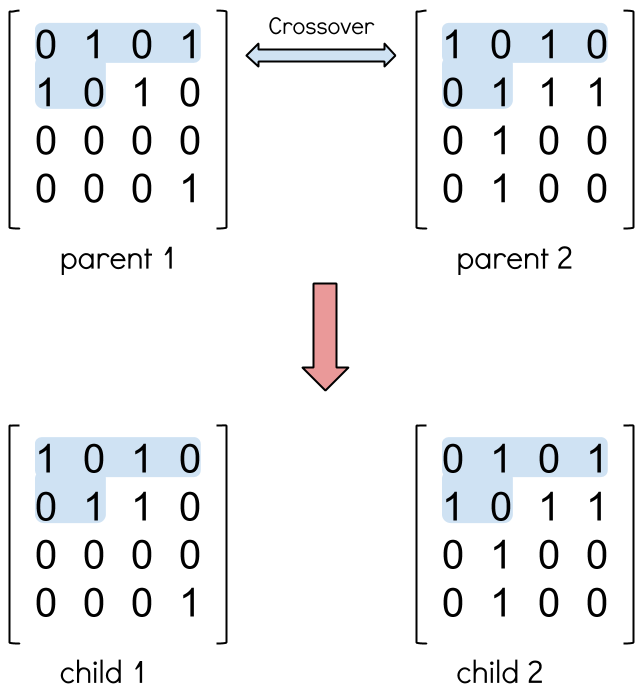
\includegraphics[width=0.3\textwidth]{pics/crossover.png}
\caption{}
\label{graph1}
\end{figure}


\subsubsection{Repair operators}
Since mutation and crossover are very likely to generate offspring that violate the constraints, therefore, 
repair operators are necessary. Normally, each constraint would has an unique repair operator 
in order to recover different types of violation.

After the process of mutation and crossover, the repair operators are examine each chromosome. 
If there is violation found in the chromosome, then it will try to repair it. 
In our problem, we have two repair operators: service number and cost.

\begin{flushleft}\textbf{Service number repair operator}\end{flushleft}
\begin{center}
		$\sum\limits_{s \in S} A_{sj} \geq 1$ \\
		service number constraint
\end{center}
The operator will go through each row of the Location Allocation matrix A, if the number of each 
service is less than one, then randomly choose one location and reverse the selected bit. 
Although the randomness does not necessarily provide an optimal solution, the computation time is 
better than exhaustively compare all solutions. 


\begin{flushleft}\textbf{Cost repair operator}\end{flushleft}
	\begin{center} 
		$\sum\limits_{s \in S} \sum\limits_{j \in J} C_{sj} \times A_{sj} \leq CostLimitation$ \\
		cost constraint
\end{center}

If the cost exceed the predefined limitation. Then the operator would iteratively check if any service has 
been deployed in more than one location. After found one service has been deployed multiple locations, 
the operator will randomly select one of them and change to zero. That means, cancel the deployment of 
that service in this location. After doing that, re-examine the chromosome, if it is still exceed the 
limitation then repeat this process until there is no redundant services or it satisfies the constraint.

This algorithm will try its best to reduce the cost regardless of other factors. Although the modified 
chromosome may end up with higher network latency, however the cost constraint has higher priority than network latency.

Worth noting that this algorithm may not provide a strictly correct solution that satisfied the constraint, 
partially because the randomly chosen of canceling deployment. On the other hand, it may also indicate that 
the predefined upper boundary of cost limitation is too low.
















This document%
\footnote{Originally written by Darrell Whitley, and only later
  modified by Marc Schoenauer, especially regarding the bibliography style,
  latest update by Hans-Georg Beyer (\today).} 
is a template which you can use to format your paper in 
preparation for publishing in the journal {\em Evolutionary Computation} 
(ECJ) and for submitting your paper to the journal. Our style file 
``ecj.sty'' is compatible with \LaTeX{} version 2e. Please note, also the 
first submission must be typeset using ECJ's \LaTeX{} style. {\em Documents 
typeset by MS Word or other office programs are not accepted.}   

Please make sure your paper is as complete and accurate as possible. You 
should typeset your paper as you would like to see it 
in its finally printed journal version (no double spacing; figures, tables 
should be embedded in the text at the most desirable locations). 

Please provide author(s) first initial and last name(s) for the even-page 
running headline. Also provide a brief paper title (45 characters/spaces or 
less) for the odd-page running headline.  See the ecjHeader section at the 
top of this document for placement of these items.

The rest of the document provides a few examples of references and 
citations, how to set up figures, discusses common problems, and provides some
general advice on writing your paper.

\begin{enumerate} 
    
\item
Give full names for authors.  (T. Bones should be Tom Bones or Thomas, 
unless your first name is a military secret and everyone calls you ``T''.)  

\item
Be sure to provide 5 to 10 keywords for your paper.  See ``keywords'' 
section above.

\item
Use the {\em Evolutionary Computation} format for references. In text 
citations should use the authors names (Smith, 1997) or ``Smith (1997) 
states ...''   The references at the back of the paper should also follow 
the {\em Evolutionary Computation} format. Using a bitex file, with
{\bf natbib.sty} and {\bf  apalike.bst}  is highly recommended. You
should then use 
\begin{itemize}
\item {\tt $\backslash$cite\{Smith\} states that \ldots} to obtain ``\cite{Smith} states that \ldots''
\item {\tt as stated in  $\backslash$citep\{Smith\}, \ldots} to obtain ``as stated in \citep{Smith} \ldots''
\end{itemize}

If you don't use natbib, be sure to follow the rules:

\begin{itemize}
\item 1 author: (Antonisse, 1989)
\item 2 authors: (Juliany and Vose, 1994)
\item multiple authors: (Reeves et al., 1990)
\item multiple citations: (Antonisse, 1989; Juliany and Vose, 1994) 
\end{itemize}


\item
If you use a bibtex file, please submit your bibtex file. In any case,
please completely 
spell out journal and institution titles.  Abbreviations may not be 
understood by all readers. Be sure to provide beginning {\em and} ending 
page numbers. Include editor(s) initials and last names(s), volume numbers, 
page ranges, publisher name and location.

See the Reference section of this paper for specific examples.

\end{enumerate}

\section{About Figures}

\begin{figure}[t]
\begin{center}
\centerline{
% \includegraphics[width=0.8\textwidth]{yourfigure.eps}
%  UNCOMMENT the above line and add yourfigure.eps
%  AND delete or comment-out the framebox
\framebox(375,50)
}
\end{center}
\caption{This is a caption below a framebox where a figure might appear.  
         Use epsfig in the {\tt $\backslash$usepackage\{epsfig,ecj...\}} 
         command to help to insure that we can process your figure.}
\label{graph1}
\end{figure}

Figures potentially cause the most serious problems when processing \LaTeX{}
files. Image files should be in EPS (encapsulated postscript) or 
PNG format (both formats produce better outcome when enlarged). However, JPEG 
can be used as well. Make sure that no unusual files are required for 
processing your figures.
The use of the ``epsfig'' or the related ``graphicx'' \LaTeX{} package is 
strongly recommended as well as the
format found in ecjsample.tex used for generating Figure 1 above.
The use of the ``includegraphics'' command is commented out in the \LaTeX{} 
file;
but you can remove the ``comment'' symbols and use the
commands shown in ecjsample.tex.\\

Make sure you provide an in-text reference to each of your figures.  An 
example is Figure 1.\\

Make sure figures are clear and fit within the margins specified in the 
style file.  Small figures with hard to read labels or hard to see lines are 
a common problem.  Also make sure that labels and terms used in figures are
defined in either the caption or the text. (It is best if they
are defined in the caption.)

\section{Common Problems and Advice}

Avoid the use of too many acronyms. You may know the meaning and 
significance of BARF (e.g., Beer, Aspirin, Recreation, and Food), but this, 
in effect, amounts to the invention of a personal language that makes 
reading your paper more difficult.  Define each acronym on its first 
occurrence it the text; thereafter, you may use the acronym alone.\\

Avoid run-on sentences.  Typically these are very hard to parse. This is 
also one of the most common problems. While you are at it, use a spelling 
tool such as ispell.\\

Avoid paraphrases - ``i.e.'', ``e.g.'', ``in other words...'', or 
parenthetical information is often unnecessarily redundant.\\

Minimize the use of prepositions and adverbs to begin a sentence (``On the other hand...'', ``Conversely...'', ``Obviously...'').  Vary your sentence 
structure.\\

Avoid using excessive supporting information/documentation.  Select only the 
material that will strengthen your paper and is relevant and necessary.\\

For paper submission and the reviewing process, only the manuscript in 
PDF format is needed. After final acceptance, we will need all your files 
in electronic form.  This package should include at least the following 
files:  .tex, .bib, .bbl, .eps, .pdf, and any 
special style files you have used to create your paper.  We also need to be 
able to \LaTeX{} and generate camera-ready PDF of your paper. Following 
the examples given in ecjsample.tex will help ensure your \LaTeX{} file can be 
processed without error.\\ 

Thank you for submitting your work to {\em Evolutionary Computation}.

\small

\bibliographystyle{apalike}
\bibliography{ecjsample}


\end{document}
